%location/filename: tex/fig/ap4.tex
%author: Anders Østevik
%Last edited: 23.05.2016
%#######--Appendix - Clock Control Software Setup --#######
%

\documentclass[main.tex]{subfiles}

\begin{document}

\chapter{Clock Control Software Setup} \label{chap:clksetup}

The Cyclone V GT kit is dependent on a number of Quartus related files, including the USB Blaster II device driver, the jtagconfig software and various device libraries included in the Quartus environment. It is therefore important to have the right version of Quartus installed for the Clock Control program to work properly. The version number of the kit (13.0.0.1 at the time of writing) corresponds to the supported version of Quartus, in this case Quartus 13.x. Newer versions of Quartus have not proven to be backwards compatible with the Cyclone V GT kit.

By using Windows, the following steps have been proven to be the best approach to make the Clock Control software work properly. The installed path to Quartus is in this case: \path{D:\Quartus_13.1}.\\

\section{Steps for Configuring Windows to run the Clock Control Software}

\begin{enumerate}\setlength{\itemsep}{10pt}
  \item Install Quartus 13.x (includes jtagconfig) together with the Cyclone V device support \cite{altera_q13}.
  \item Set appropriate environment variables. In Windows, this should be set automatically.
  \begin{itemize}\setlength{\itemsep}{10pt}
      \item PATH -- \path{"D:\Quartus_13.1"}
      \item QUARTUS\_ROOTDIR -- \path{"D:\Quartus_13.1\quartus"}
      \item SOPC\_KIT\_NIOS2 -- \path{"D:\Quartus_13.1\nios2eds"}
    \end{itemize}
  \item Connect the Cyclone V board to the \gls{pc} using USB Blaster II (Refer to the manual for instructions on how to install the USB Blaster II \cite{altera_usb}).
  \item In Command Prompt (cmd.exe):
  \begin{itemize}\setlength{\itemsep}{10pt}
      \item Navigate to the "board\_test\_system" folder located inside the Cyclone V kit.
      \item run "jtagconfig" and confirm connection with the board. If the Command Prompt cannot find jtagconfig, navigate to \path{D:\Quartus_13.1\quartus\bin} using a file explorer and manually start jtagconfig.exe from there
      \item run "java -Djava.library.path=\path{"D:\Quartus\_13.1\bin"} -jar clk\_cont.jar". The library path is to ensure that the Java environment have access to the appropriate Quartus libraries it needs to connect with the board.
    \end{itemize}
\end{enumerate}

If done correctly, the Clock Control software will start up and display "Connected to the target" in the message window. The default output frequency of the $Si570$ oscillator is $100~\mega\hertz$. The output frequency is calculated using the following equation:

\begin{equation}
%\[
    f_{out} = \frac{f_{XTAL} \times RFREQ}{HSDIV \times N1}
%\]
\end{equation} 

, where $f_{XTAL}$ is a fixed frequency of $114,2857~\mega\hertz$; RFREQ is a floating point 38-bit word; and HSDIV and N1 is the output dividers \cite{si570}. The parameters are determined by the Clock Control software based on the user typed frequency. The parameters are then sent serially via the USB Blaster II to the $Si570$ chip, where the above formula is used to set the internal registers for the new frequency.
Figure \ref{fig:clk_cont120} shows the Clock Control software after a new frequency of $120~\mega\hertz$ is set. 

\begin{figure}[H] % H(strictly put HERE > h!)
\begin{center}
% h(here), !(force), t(top), b(bottom), p(on extra page)
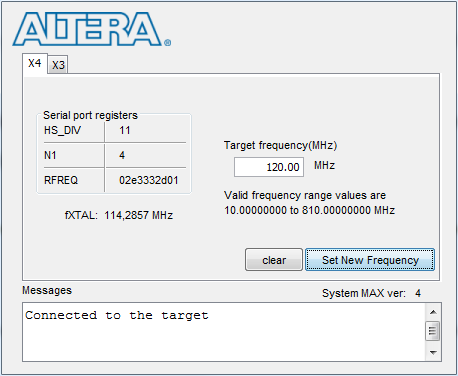
\includegraphics[scale=0.8]{../img/clk_cont120}  \\[0.1 cm]
\caption{Clock Control software by Altera used to program the $Si570$.}
\label{fig:clk_cont120}
\end{center}
\end{figure} 

The $Si570$ is volatile, meaning that the output frequency is reset back to $100~\mega\hertz$ if power is lost. The procedure must therefore be repeated every time the \gls{fpga} is powered on.\\
To confirm correct operation, a quick measurement of the output clock was done using an oscilloscope. Figures \ref{fig:tek100} and \ref{fig:tek120} shows the output frequency, before and after configuration.\\

\begin{figure}[H]
   \begin{floatrow}
     \ffigbox{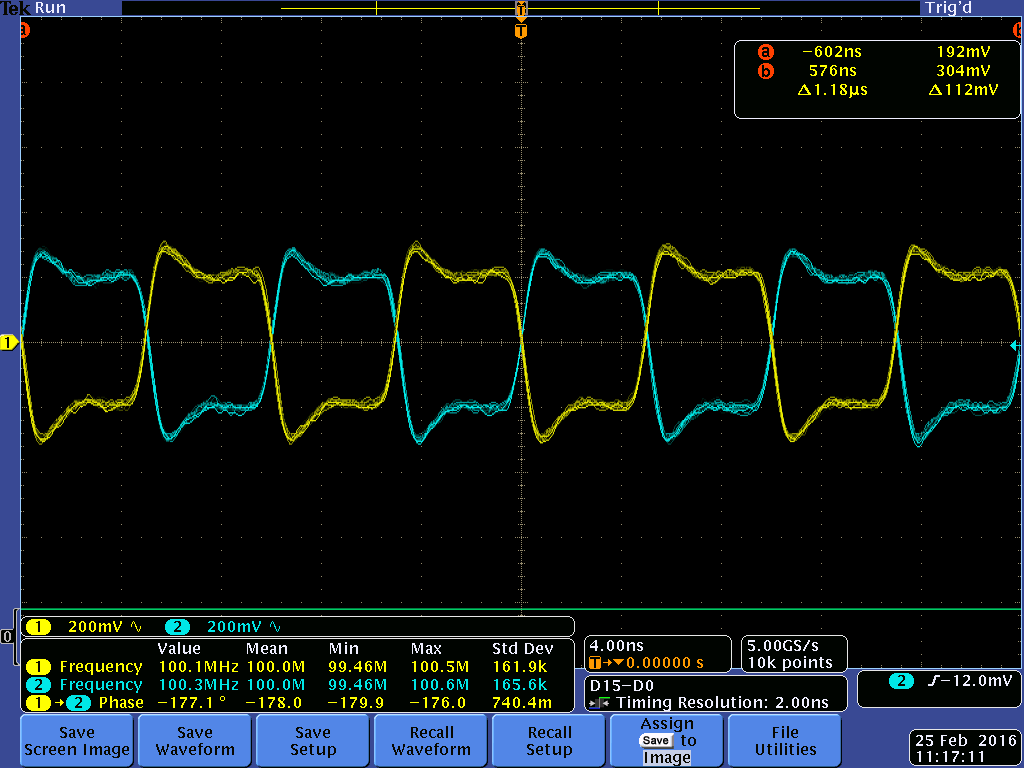
\includegraphics[scale = 0.2]{../img/20160226_tek100}}{\caption{$Si570$ Before configuration: 100 MHz.}\label{fig:tek100}}
     \ffigbox{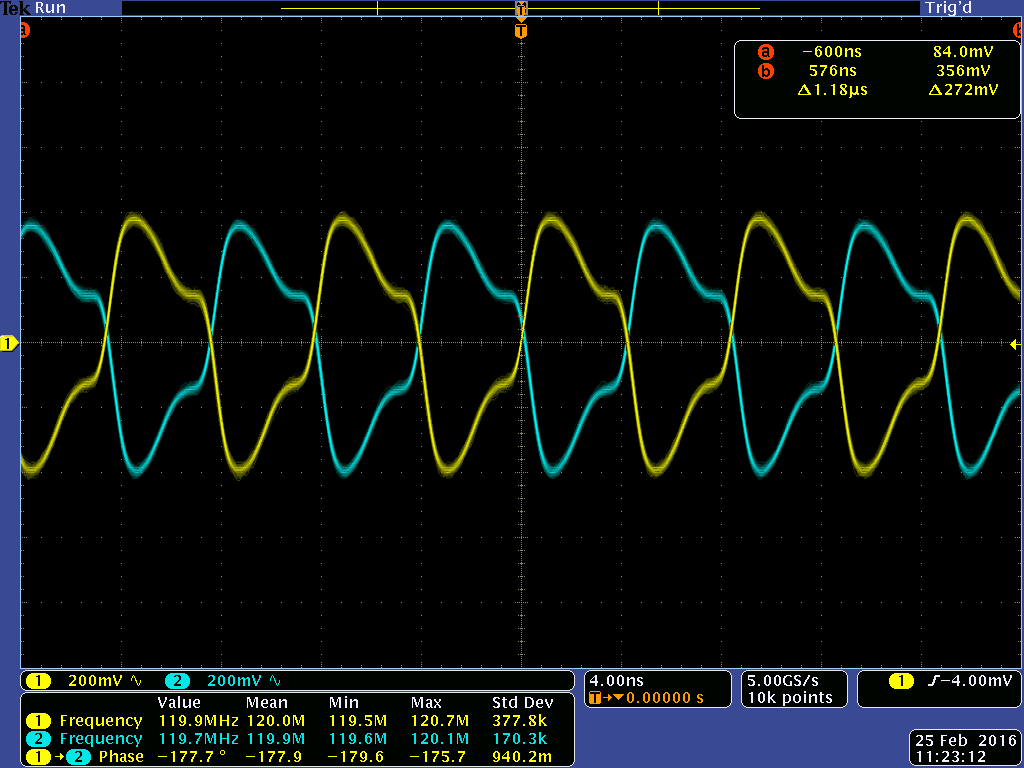
\includegraphics[scale = 0.2]{../img/20160226_tek120}}{\caption{$Si570$ After configuration: 120 MHz.}\label{fig:tek120}}
   \end{floatrow}
\end{figure}

\end{document}
